\documentclass{article}
\usepackage[utf8]{inputenc}
\usepackage{graphicx}
\graphicspath{{../}}
\title{\textbf{Using Natural Language Processing to Analyse the Shape of Stories}}
\author{
Luca Davies \\ BSc. (Hons.) Computer Science}
\date{March 2020}

\usepackage{natbib}
\usepackage{graphicx}
\usepackage{float}

\begin{document}
\maketitle
\newpage
\section*{Declaration}
    I certify that the material contained in this dissertation is my own work and does not contain unreferenced or unacknowledged material. I also warrant that the above statement applies to the implementation of the project and all associated documentation. Regarding the electronically submitted work, I consent to this being stored electronically and copied for assessment purposes, including the School’s use of plagiarism detection systems in order to check the integrity of assessed work. \\
    I agree to my dissertation being placed in the public domain, with my name explicitly included as the author of the work. \\
    
    \noindent
    Name: \\
    Date:
\newpage
\section*{Abstract}
    This report examines the application of Natural Language Processing and Sentiment Analysis to fictional texts in an attempt to summarise narrative arcs as a curve on axes of time against positive/negative sentiment. VADER is used to process text for sentiment analysis and further experimentation is carried out to analyse how suitable VADER may be for this task. Corpora was mainly sourced from Project Gutenberg. A tool was developed to carry out a range of experiments on sentiment analysis that employed VADER as it's sentiment analysis engine. Experimentation was carried out in the context of sentiment analysis around the following topics: the coarseness of sentiment analysis; the accurarcy of VADER at sentence level via hand-tagging; sentiment analysis vs. analysis by human readers; early-modern English vs. modern English; Shakespearean comedies vs. tragedies. It was discovered that a more powerful and versatile sentiment analysis engine would likely be needed to produce more readable curves and that a more flexible tool would prove useful for processing different text styles, such as scripts.
\newpage
\tableofcontents
\newpage
\section{Introduction}
    \subsection{Overview}
        Writer Kurt Vonnegut suggested at various points in his career that all stories may be categorised into a relatively small number of basic archetypes based upon the emotional ups and downs experienced within the narrative. He gave each of these novel names such as Man-In-Hole and Boy-Meets-Girl as a simple reference for each. \cite{vonnegutLecture}

        Literature is one of the defining features of the human race. No other creature on Earth can writes, let alone writes about itself. Humanity takes this a step further again, making up fictitious stories, some rooted in reality, some with no basis at all in which we dream and imagine worlds and situations that may never be possible to achieve. Through written word we express emotion. All emotions, happiness, sadness, anger and fear; love, hate, awe and grief – everything humans can feel, we write about. We create characters to express and receive these emotions, they act as vehicles to transfer their feelings to a reader. With all this freedom to write and create without bound, are we actually as free as we perceive?

        Vonnegut suggests that all stories are members of one of a very small number of categories of story that define roughly how the emotional progression of that story pans out. Do writers naturally and unknowingly write literature that falls into these types or is each story as unique as the next, taking its readers along its own path as they go?

        This concept and these questions drew me toward this project proposal. Not only is it a fascinating endeavour to map the emotions of a novel, but as an exploration of the freedom of writers to convey emotions and of how humans often generate categories and groups without even trying.

        With the high-level view clarified, it's important to note the tools within natural language processing that are relevant, namely that in this study, sentiment analysis takes the spotlight. Emotional analysis is a more in-depth field that shifts focus toward the psychological analysis (\cite{sentimentVsEmotionAnalysis}) and employs machine learning and artificial intelligence to further predict and understand the emotions presented in text.
    \subsection{Motivation}
        At it's core, this study is novel. It is interest driven - to attempt to show that stories can be categorised in a very simple and easy manner based upon the emotional arcs they lead readers across is an interesting new way to sort fiction. There may not be any significant \emph{need} to categorise literature in this way, however it has the potential to lead to further studies.
    \subsection{Aims \& Objectives}
        The aims of this report are as such:
        \begin{itemize}
            \item Design and develop an application to process a range of corpora to produce a graphing of the emotions during its literary course
            \item Analyse a range of corpora for compliance with Kurt Vonnegut’s theories and story shapes
            \item Otherwise attempt to identify trends the texts processed
            \item Study the produced graphs and compare expectation surrounding the source text
        \end{itemize}
\newpage
\section{Background}
    \subsection{Overview}
        This chapter will examine and summarise existing literature and studies in this area and topic. That is, natural language processing and sentiment analysis as a tool for extracting statistical data that describe emotions in (mainly) fictional works of literature.

        The processes involved for finding useful information included searching for online articles and pre-existing projects while searching libraries to use in the implementation, Google Scholar, Lancaster University Library OneSearch and Kurt Vonnegut’s own lectures on this topic.

        Existing projects will help to prove the developed application is performing up to standard (or not) and can be used as a side-by-side comparison of literature processed for this report and by these projects as well as to examine the processing of literature unavailable for the purposes of this report.
    \subsection{Natural Language Processing \& Sentiment Analysis}
        Natural Language Processing (NLP) is a very broad field concerned with, at a high level, the understanding of human language by computers. It fuses linguistics with computer science to not just parse but to \emph{understand} human language, to understand it in such a way that meaning can be deduced and emotion and sentiment can be extracted, even when not fully clear.

        Via the beginnings of machine translation, NLP has existed as a research field for decades, even before the current name was coined. Breakthrough projects like ELIZA made progress in the field, but it wasn't until the 1980s that statistical methods began to be used. Prior to this, large sets of hand-written rules governed how NLP systems worked, which, although sometimes effective, limited the overall progress to the manual effort put into the models and rules. In modern NLP toolkits, models are still prevalent, but instead of them being assembled by hand, they are often formed using machine learning techniques based upon employing training data, test data and then real language data.

        Sentiment Analysis (SA) is a subfield of NLP that focuses on extracting and subsequently quantifying opinion and sentiment around a topic simply by analysing text. SA is a particularly new field, and has so far mainly be used on corpora that is factual and descriptive: product/movie reviews and social media to gauge general public opinion.
    \subsection{Kurt Vonnegut on ``The Shape of Stories''}
        Vonnegut described a number of potential story types as displayed below in figure something. He suggested that all stories fit into a very small number of categories, and moreover, that stories from different cultures around the world may generally trend toward different story types compared to elsewhere. In his lecture on the topic Vonnegut draws out the curves of some well known novels and stories to demonstrate his meaning. Drawing distinct curves with very defined turning points and changes in direction that match up with points in the given literature.
        \begin{figure}
            \centering
            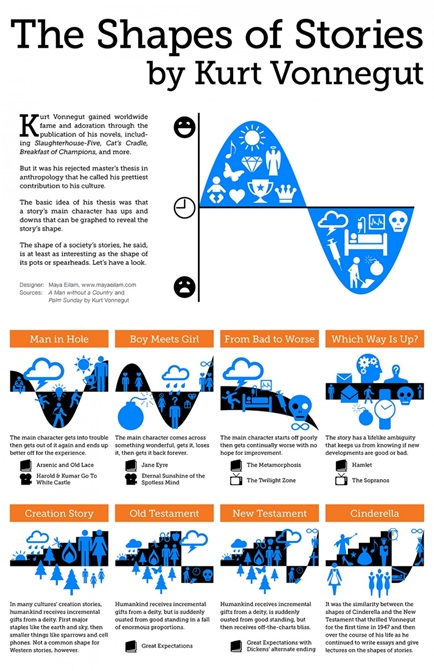
\includegraphics{Misc/VonnegutShapes}
            \caption{Vonnegut's Story Types}
            \label{fig:storyTypes}
        \end{figure}
    \subsection{The Hedonometer Project}
        The Hedonometer project was established to gauge happiness, the world over, starting with Twitter and other social media outlets. The project’s scope has since widened to process corpora direct from books, film scripts, news outlets and other foreign language literature.
\newpage
\section{Sentiplot Tool}
This section will detail the design and implementation of the tool used to carry out this study, \emph{Sentiplot}. 
    \subsection{Languages \& Libraries}
    This section briefly discusses the choice of programming language and NLP/SA tools used in the Sentiplot tool.
        \subsubsection{Top-level Language}
        When selecting which language would be most appropriate to use for this project, my major considerations were my prior knowledge of potential languages and their ease of creation of a pleasant user interface. Availability of NLP tools in each language was also to be considered, but as the end implementation shows, this was not imperative due to cross-platform and cross-language capabilities of the chosen combination of languages and tools.

        A listing of considered languages follows:

        \begin{itemize}
            \item Java
            \begin{itemize}
                \item Strong language knowledge and familiarity
                \item JavaFX and Swing available for interfaces
                \item Native language of Stanford CoreNLP
            \end{itemize}
            \item Python
            \begin{itemize}
                \item Very limited language knowledge
                \item No knowledge of interface building
                \item Native language of industry standard NLTK
            \end{itemize}
            \item C\# (with .NET)
            \begin{itemize}
                \item Strongest language knowledge and familiarity
                \item Extreme ease in creating interfaces via Windows Form using Visual Studio
                \item Cross-platform variants of CoreNLP and VADER available via simple packages
            \end{itemize}
        \end{itemize}
        Taking all these points into consideration C\# was selected, due to its pros specific to myself and the availability of non-native libraries via APIs. This permitted me to use the full Microsoft Visual Studio suite for development, including the Windows Forms designer.
        \subsubsection{Natural Language Processing Tools}
        Various tools across a wide array of languages are freely available to provide standard NLP functions and advanced processing capabilities.

        Initially a full CoreNLP pipeline was employed to process corpora but this proved to be extremely slow, loading around 2 gigabytes of models very slowly into memory before even processing anything. The pipeline was modified to tokenise and sentence-split only and the actual sentiment analysis was performed by VADER.

        Both the CoreNLP and VADER libraries are non-native to C\# but have easy to use APIs for direct manipulation of their types and methods outside of their native environments. CoreNLP has an in-house developed API for C\# and VADER has a third-party API called \emph{VADERSharp}.
    \subsection{Implementation}
        \subsubsection{Structure}
            The application is written in C\# .NET interfacing with both Java and Python libraries via APIs as detailed in the previous section. Windows Forms was chosen for the interface as a quick and easy to build platform, stable on Windows with seamless integration into C\# and the .NET framework.

            The application is composed of two forms, each with their designer code. The first allows the user to select a file to load text from and set processing granularity. The second presents the results of the analysis in multiple ways and provides facility to save these results as images of the output graphs.
        \subsubsection{Sentiplot Form (Main Form)}
            This is the main form for the application. It is loaded on start-up and contains all needed information or otherwise calls other classes to complete its task.

            Its key functions include:
            \begin{itemize}
                \item Initialising the CoreNLP pipeline ot tokenise the input text
                \item Generating an OpenFileDialog object to allow the user to select a \emph{.txt} or \emph{.html} file
                \item Parsing the content of the input file to prepare it for processing using regular expressions and simple character-based splitting
            \end{itemize}
        \subsubsection{ResultsViewer}
            This form displays the results of VADER's processing of the input text. It displays a graph of the entire text from start to finish, a full list of all tokenised sentences and their associated sentiment scores (in tabular form) and individual graphs for each chapter in the text (HTML file only).

            \begin{itemize}
                \item Handling the output data and feeding it into the main chart and table
                \item Allow hiding/showing of each different type of sentiment score for the main graph
                \item Dynamically producing more tabs on the form to show each successive group of five chapters
            \end{itemize}
    \subsection{User Interface}
        The implemented interface did not need to be excessively complex or particularly appealing as it mainly served to function as a harness to conduct the study, with more importance placed on the code-behind and results.

        To provide quick results and ease of programming, I used the Windows Forms suite to produce a visually simple but functional interface. It has two screens: a screen to load the desired text to be processed and to set the granularity of the analysis, and a screen to present the processed results. The following sections provide an overview of these screens.
    \subsubsection{Text Selection \& Options}
    Figure \ref{fig:sentiplot} shows the main presented screen, after having loaded an HTML file (Hamlet in this case) which has been parsed to produce plaintext, having stripped out all the unneeded HTML tags.
        \begin{figure}[H]
            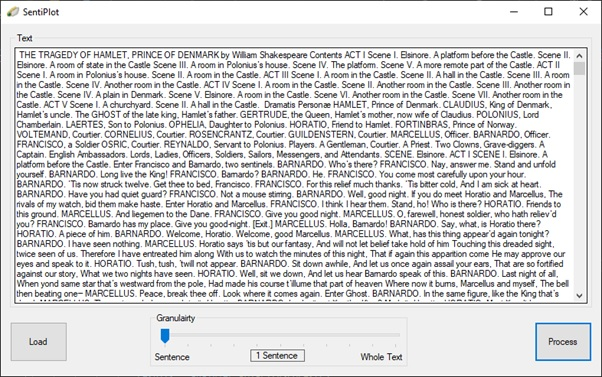
\includegraphics[width=1\textwidth]{Misc/sentiplot}
            \caption{Main Sentiplot window}
            \label{fig:sentiplot}
        \end{figure}
    \subsubsection{Results Display}
        Figure \ref{fig:resultsviewer} shows the results screen for Hamlet, initially showing the graph of the entire text. The maximum and minimum points are labeled with the start of the related sentence. Hovering the mouse over these labels shows the entire sentence or sentences that produced that datapoint.

        For every sentence analysed VADER returns four sentiment scores: positive, neutral and negative (each holding a -1 to 1 score regarding match to that sentiment), and compound which acts as a single representation for the sentiment in the sentence parsed. Each of these scores have their own graph which may have their visibility toggled on and off with the check boxes in the bottom left. (Default is compound alone, as it proved the most indictive of sentiment, as advised by VADER documentation.) This graph can be saved to a JPG by clicking the save button.
        \begin{figure}[H]
            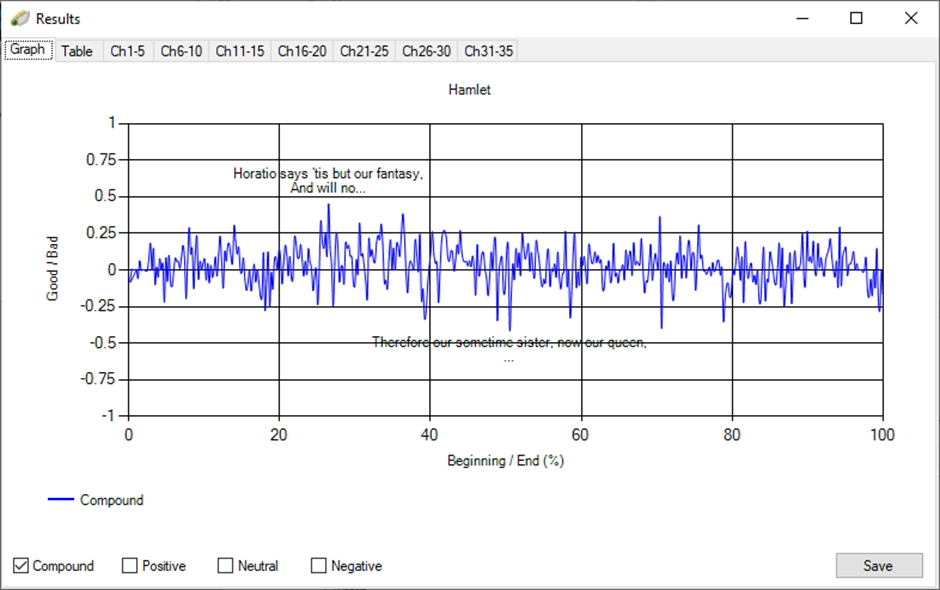
\includegraphics[width=1\textwidth]{Misc/resultsviewer}
            \caption{ResultsViewer window}
            \label{fig:resultsviewer}
        \end{figure}
        Figure \ref{fig:resultstable} shows the Table tab of the results screen. This simply lists each individual sentence token in the input with VADER’s output value for the four scores mentioned previously. The table’s default ordering in by sentence index, or the chronological order in the text, but the it may be order by any of the fields shown.
        \begin{figure}[H]
            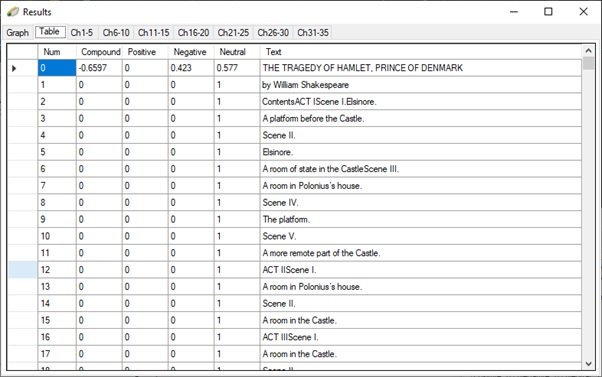
\includegraphics[width=1\textwidth]{Misc/resultstable}
            \caption{ResultsViewer window showing table}
            \label{fig:resultstable}
        \end{figure}
        Figure \ref{fig:resultschapters} shows one of the chapter tabs from the results screen. Each of graphs the compound sentiment score of up to 5 chapters from the processed text. Again, maxima and minima are labeled with their relevant sentence(s), expandable by hovering the mouse over the label.
        \begin{figure}[H]
            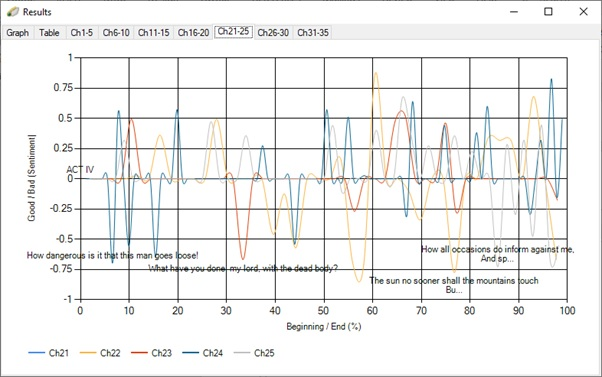
\includegraphics[width=1\textwidth]{Misc/resultschapters}
            \caption{ResultsViewer window showing chapter graphs}
            \label{fig:resultschapters}
        \end{figure}
\newpage
\section{Experimentation}
The following section covers the various experimentation and analysis carried out using Sentiplot as a tool for Sentiment Analysis and graphing accordingly.
    \subsection{Analysis Block Size}
        Sentiplot incorporates one primary setting for its analysis of texts: the granularity slider. This allows the user to select varying degrees of granularity for the produced graphs (as a percentage of the text being analysed). This allowed analysis of texts at a number detail levels to find which produced the most obvious curves to conform with Vonnegut's story curves. This may have introduced a small amount of positive-results bias, accepting those granularities that appear most curve-like for a given text instead of what may have actually reflected the curve of the text.

        The following options are provided:
        \begin{itemize}
            \item 1 sentence
            \item 0.1\%
            \item 0.2\%
            \item 0.5\%
            \item 1\%
            \item 2\%
            \item 5\%
            \item 10\%
            \item 25\%
            \item 50\%
            \item 100\%
        \end{itemize}
        This set of experiments varied the analysis blocksize for a given text and compared the output graphs for the entire text with a view to identifying a specific curve for the text. The comparison is qualitative, employing only human visual reference as opposed to any mathematical function. The purpose of this part of the study was as a forerunner to further analysis and experimentation to find the best setting or the best range of settings for either specific or generically for all texts to produce a coherent sentiment curve.
        \begin{figure}
            \includegraphics[width=0.5\textwidth]{Figures/Blocksize/Cinderella/cinderellaGran}
            \centering
            \caption{Each graph shows the result of decreasing the granularity of analysis and show how there appears to be a sweet spot. In this case, four of the highest options summed only a single sentence due to short length of the text. Only one of these has been included.}
            \label{fig:cinderellaGran}
        \end{figure}
        Figure \ref{fig:cinderellaGran} show the differing graphs that may be produced by changing the granularity.

        VADER is designed for parsing short lengths of text (less than 140 characters, as per a Tweet), so in order to produce more coarse graphs than single-sentence, VADER is still fed text on a per-sentence basis with the results summed up to \emph{N} sentences where \emph{N} is the corresponding number of sentences for a given granularity setting for a given text. The relevant data point is then plotted \emph{N} sentences beyond the previous (i.e. at the end of the analysed block).

        By default, every sentence of the text is plotted as its own point. This gives highly detailed graph but it very difficult to discern any sort of shape. Sentence to sentence, sentiment can vary wildly from the most negative in one to the most positive in the next (context and corpus dependent). Due to this, the resultant graph is highly spiked and difficult to garner information from.

        By contrast, using the more coarse options of 25\% and upward produce graphs that do show a clear line, however, at this level of coarseness, the data is compressed so much so that much of the detail is lost, smoothing the curve that should be shown beyond useful limits.

        Through trial-and-error experimentation, the ideal setting was found to lie between 0.2\% and 2\%, erring toward the 2\% for most texts.

        
        With this being said, it's possible, that a different tool may have been better suited to this task than VADER due to it's native design choice to parse text the length of Tweets, not entire corpora.
    \subsection{Hand Analysis Vs. VADER}
        This test was performed by selecting a 100 random sentences from two texts (Macbeth and Cinderella), analysing them each individually by hand and estimating a combined positive/negative sentiment score in the same range as that produced by VADER. I attempted to avoid trying to emulate the way VADER would process the text, instead scoring each sentence as I would as a reader of the text: "Would I feel positively and negatively after reading this sentence?" or, similar.
        
        The motivation behind this was to understand if VADER's output results were trustable, totally incorrect, or somewhere in the middle. 

        VADER also lacks any context processing - it cannot understand running themes in texts in order to better understand the sentiment behind that which is being said.
    \subsection{Reader Analysis \& Reflection}
    \label{subsec:reader}
        This section covers the analysis of a range of Shakespeare plays by human readers (mostly identified to be Theatre and/or Literature students) and their personal comparison of the the Sentiplot output with their own expectations of what a graph of a given play should be. The goal here was to bring a human element to the reviewing of Sentiplot and VADER. A brief background of the study was given to each person who answered any of the questions provided. Some asked further questions and subsequently commented on the techniques used for analysis and graph production.
        \subsubsection{Reader Analysis}
            Readers were first asked if they felt they knew each play well enough to attempt to plot major emotional events from each on a graph. Consequently some participants opted to answer questions only on a few of the six presented plays. In total, 22 result sets to compare a human's analysis with VADER were gathered.

            Each participant was given a blank set of axes (with the same scale as was used for VADER's results). They were asked to draw what they thought a curve of each play would look like, based upon any and all major events they can recall. They were then asked to label and/or explain any notable troughs and peaks in their curves. A small selection of the curves drawn are shown in figure \ref{fig:readerVsVader}, paired with the corresponding output form VADER.
            \begin{figure}
                \includegraphics[width=1\textwidth]{Figures/Survey/readerVsVader}
                \centering
                \caption{Readers (top of each pair) in general drew curves bearing little to no similarity to those produced by VADER (bottom in each pair)}
                \label{fig:readerVsVader}
            \end{figure}
            In general, all the curves drawn by participants were grossly different to the VADER output for the same texts. All VADER's curves stayed mostly in the range of +/-0.25 on the Sentiment axis, whereas most participants drew curves using nearly the full extent of the y-axis. This is not to say that VADER doesn't register any sentences as reaching the more extreme values: when examining the per-sentence scores in the table view, it does, but these values get flattened when they are grouped together. On closer inspection, taking Macbeth as an example, approximately 30\% of the sentences were outside the +/-0.25 range, however  just over 60\% of those \emph{within} the range were zeros, registered by VADER as completely neutral sentences. When taking averages, these high volumes of zero-scored sentences will have reduced the impact on the output graph of higher scores greatly.

            Even with this failure, attempting to look at relaitve differences along the two curve sets (those drawn, and those produced by VADER) still doesn't yield much similarlity. The only immediately obvious correlation is, again, in Macbeth where both VADER and a participant show a sharp dip at around the halfway mark (labeled on the drawn curve as "murder"). This is nearly the only obvious match, however.
    \subsection{Shakespeare: Comedies Vs. Tragedies}
    \label{subsec:comVsTrag}
        As mentioned in section \ref{subsec:reader}, Shakespeare plays have been a key source of analysis text. These have generally yielded somewhat restricted graphs. The motivation for these tests came from the thought to force the ability to tell apart different plays by their genre. Namely to comedies \emph{should} show generally more positive curves and similarly, tragedies \emph{should} show more negative curves accordingly. To attempt to display this, three comedies (\emph{Twelfth Night, The Tempest, A Midsummer Night's Dream}) and three tragedies (\emph{Macbeth, Hamlet, Romeo \& Juliet}) were processed to give their repsective graphs. There is some debate on the specific genre of \emph{The Tempest}, it now often being referred to as a \"late romance\", a subsection of Shakespeare's comedies leaning more toward a \"tragicomedy\" in genre. Nonetheless it ought to still produce a difference in curve to that of the three tragedies.
    \subsection{Early Modern Vs. Modern English}
        VADER is not trained to work on the likes of formal literature. In fact, it is trained to work on highly modern and informal text, to such an extent that it understands and can analyse Internet slang and emoji. Due to this fact, this experiment was carried out to test of VADER was able perform equally or at all as well on a different form of English, that being the Early Modern English found in the Shakespeare plays processed for sections \ref{subsec:reader} and \ref{subsec:comVsTrag}.
\newpage
\section{Conclusion}
\newpage
\bibliographystyle{plain}
\bibliography{ref}
\end{document}
